\newpage % Rozdziały zaczynamy od nowej strony.
\section{Opis rozwiązania}
Rozwiązanie zadania konkursowego zostało w całości zaimplementowane w języku Python w wersji 3.8. Najważniejsze biblioteki jakie zostały wykorzystane w rozwiązaniu to:
\begin{enumerate}
\item \texttt{torch} do obsługi danych i modeli.
\item \texttt{albumentations} do przetwarzania obrazów.
\item \texttt{pytorch\_lightning} do trenowania i ewaluacji modeli.
\item \texttt{segmentation-models-pytorch} do budowy modeli.
\item \texttt{neptune} do monitorowania przebiegu treningu i ewaluacji.
\end{enumerate}
\subsection{Zbiór danych}
Do wstępnej obróbki zbioru danych wykorzystano skrypty dostarczone przez organizatorów konkursu razem z rozwiązaniem \textit{baseline} w niezmienionej postaci. Przetwarzają one adnotacje w formacie GeoJSON na obrazy w formacie TIFF i rozdzielczości identycznej jak odpowiadające im zdjęcia. Dla jednej pary zdjęć (przed i po katastrofie) generowane są maksymalnie cztery obrazy:
\begin{enumerate}
\item Jednokanałowa maska budynków o wartościach $0, 1$.
\item Jednokanałowa maska dróg o wartościach $0, 1$.
\item Jednokanałowa maska dróg o wartościach 0 -- 7, odpowiadających różnym rodzajom dróg. Nieużywana w tej pracy.
\item Czterokanałowa maska budynków i dróg po katastrofie o wartościach $0, 1$. Kanały odpowiadają następującym obiektom, w kolejności: niezniszczony budynek, zniszczony budynek, niezniszczona droga, zniszczona droga.
\end{enumerate}
Po przetworzeniu zbiór danych zawierał 801 par zdjęć z kompletem masek dróg i budynków przed i po katastrofie. Według podziału narzuconego w konkursie 679 par znalazło się w zbiorze treningowym i 122 w zbiorze testowym.\\
\begin{figure}[h]
\centering
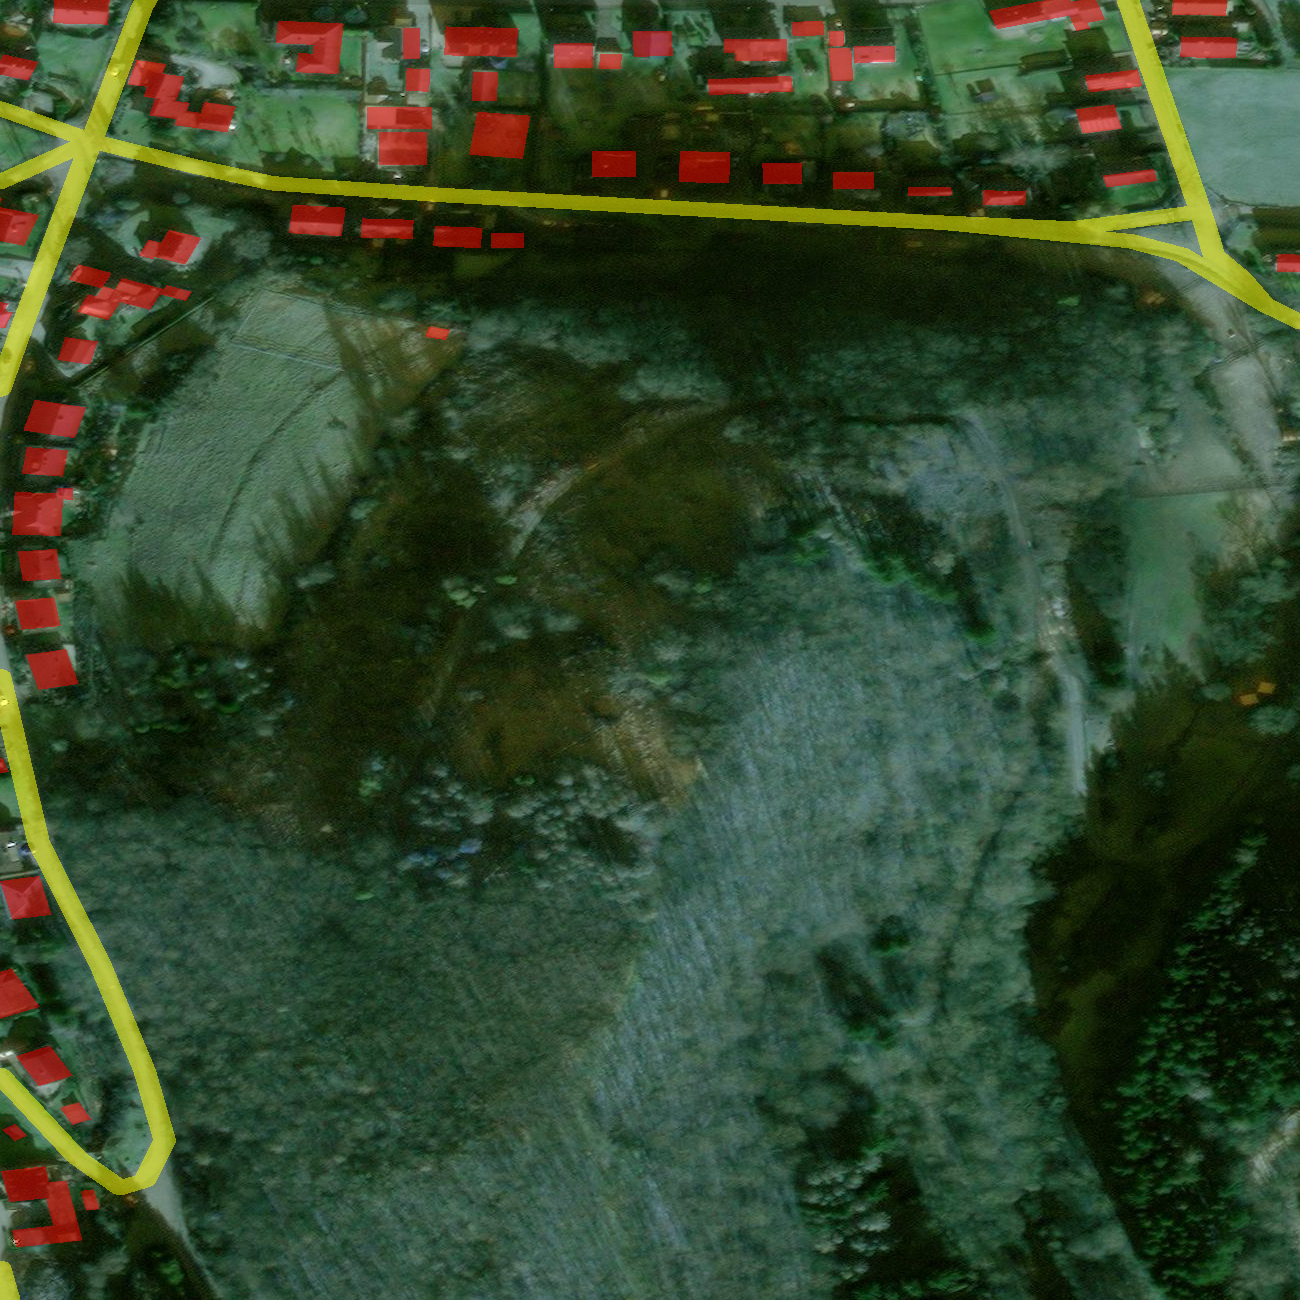
\includegraphics[width=7cm,height=7cm]{rysunki/10500500C4DD7000_0_30_69_PRE.png}
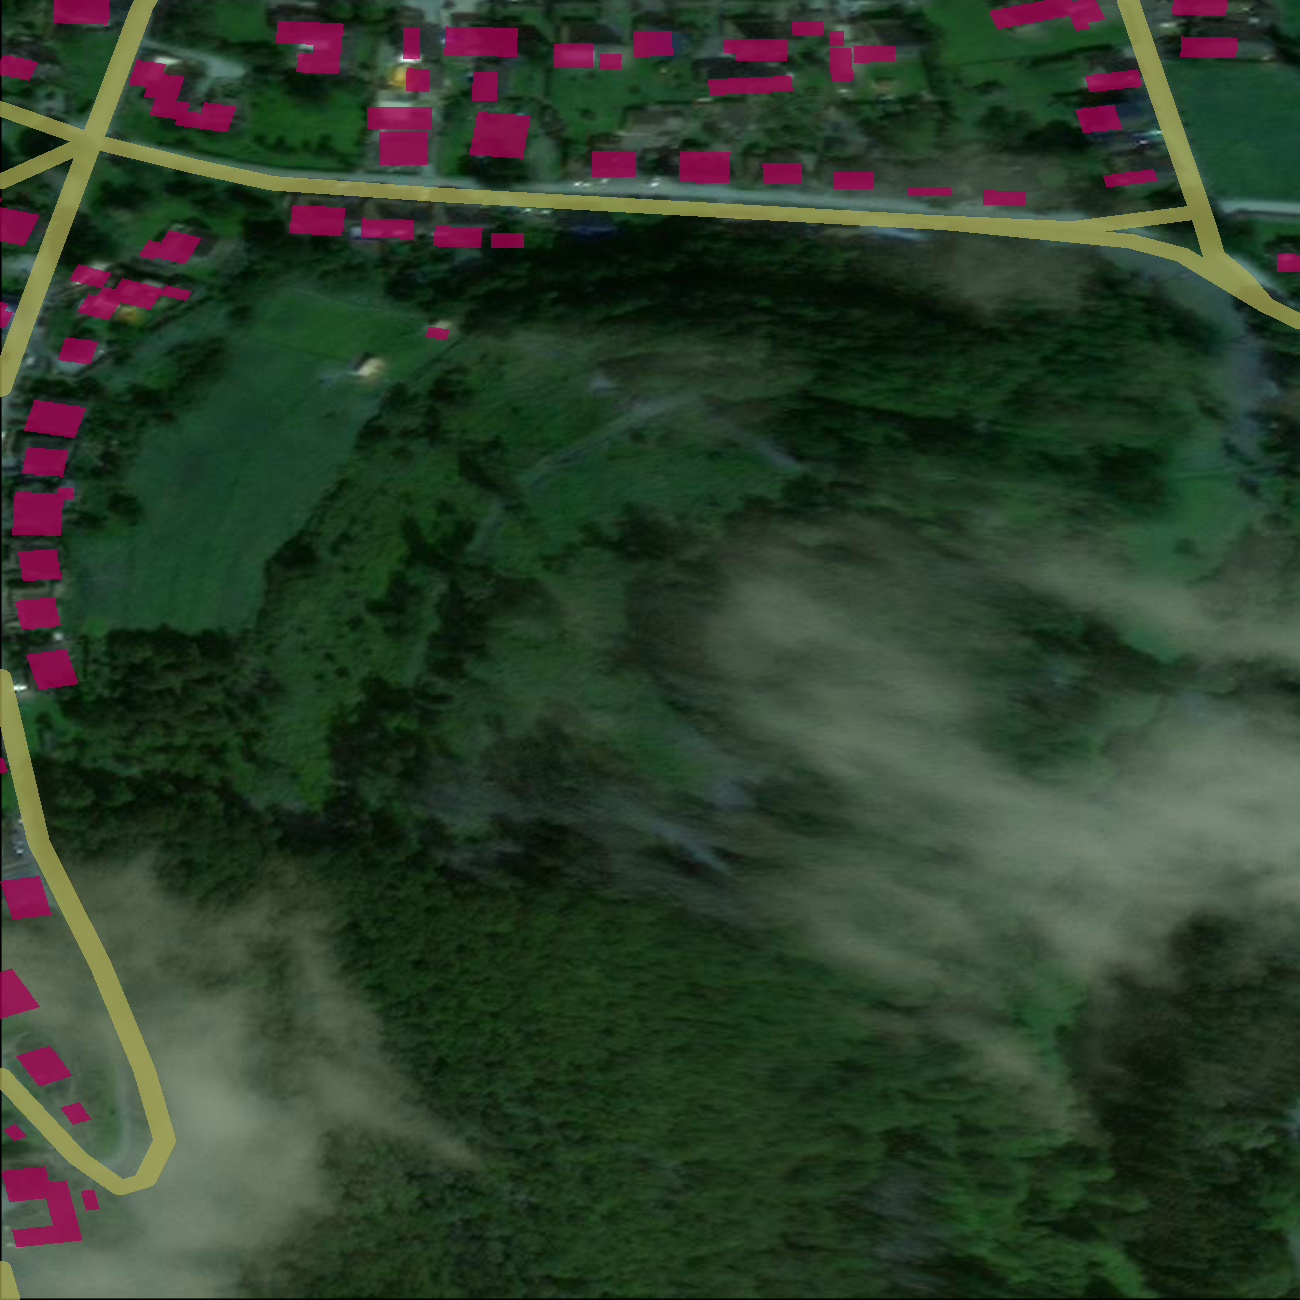
\includegraphics[width=7cm,height=7cm]{rysunki/10500500C4DD7000_0_30_69_POST.png}
\caption[Wizualizacja danych]{Przykładowa para zdjęć ze zbioru danych z adnotacjami. Wszystkie obiekty na zdjęciu po prawej są sklasyfikowane jako zniszczone.}
\end{figure}
Zdjęcia sprzed katastrofy miały rozdzielczość $1300\times 1300$ pikseli, natomiast zdjęcia po katastrofie miały różne rozdzielczości. Aby efektywnie używać ich jako wsadu do modeli o różnych architekturach, zaimplementowano skalowanie wszystkich obrazów i masek po ich wczytaniu do tej samej rozdzielczości. W eksperymentach ustalono tę rozdzielczość na $1024\times 1024$ piksele.
\subsection{Augmentacja danych}
Ze względu na mały rozmiar zbioru danych, kluczowe znaczenie dla rozwiązania miała augmentacja danych treningowych. 
\subsection{Trening i ewaluacja}

\subsection{Eksperymenty}

